% Non-self-intersecting parameterized curve; both Bezier pieces have
% derivative 3*(0.4,0.5) at sigma(t), parallel to the velocity arrow.
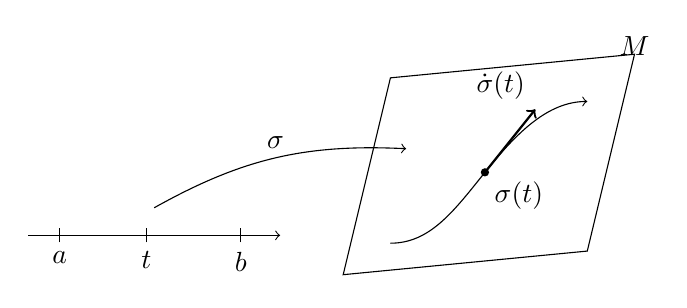
\begin{tikzpicture}
	\draw[->](0,0)--(3.2,0);\foreach \x/\t in {.4/a,1.5/t,2.7/b}{\draw(\x,-.09)--(\x,.09)node[below=5pt]{$\t$};}
	\draw[->](1.6,.35)to[bend left=16]node[above]{$\sigma$}(4.8,1.1);
	\draw(4,-.5)--(4.6,2)--(7.7,2.3)--(7.1,-.2)--cycle;\node at(7.7,2.4){$M$};
	\draw[->](4.6,-.1)..controls(5.1,-.1)and(5.4,.3)..(5.8,.8)
		..controls(6.2,1.3)and(6.6,1.7)..(7.1,1.7);
	\fill(5.8,.8)circle(1.5pt)node[below right]{$\sigma(t)$};
	\draw[->,thick](5.8,.8)--(6.44,1.6)node[above left]{$\dot\sigma(t)$};
\end{tikzpicture}
